% !TeX root = RJwrapper.tex
\title{\pkg{NTS}: An \bf{R} Package for Nonlinear Time Series Analysis}
\author{by Xialu Liu, Rong Chen, and Ruey Tsay}

\maketitle

\abstract{
Linear time series models are commonly used in analyzing dependent data and in forecasting.
On the other hand, real phenomena often exhibit  nonlinear behavior and the observed data show nonlinear dynamics. This paper introduces the  {R} package \pkg{NTS} that offers various computational tools and nonlinear models for analyzing nonlinear dependent data. The models used include threshold autoregressive models, autoregressive conditional mean models with exogenous variables, functional autoregressive models, and state-space models. Users can also evaluate and compare the performance of different models and select the best one for prediction. Furthermore, the package implements flexible and comprehensive sequential Monte Carlo methods (also known as particle filters) for modeling non-Gaussian, nonlinear processes. Several examples are used to demonstrate the capabilities of the \pkg{NTS} package.

}
\section{Introduction: nonlinear time series analysis in R}\label{sec:intro}


Time series analysis investigates the dynamic dependence of data observed over time or in space. While linear time series analysis has been extensively studied in the literature with many software packages widely available, nonlinear time series analysis only attracts limited attention. In particular, there is relatively little effort devoted to the development of software or packages for analyzing nonlinear time series data. The \pkg{NTS}, a recent {R} \citep{R} package, provides a number of functions for simulating, analyzing, and predicting nonlinear time series data. The models available include univariate and multivariate threshold autoregressive models, conditional intensity models,
nonlinear state-space models, and functional time series models. The package also features various nonlinearity tests and sequential Monte Carlo methods. The package is now available from the Comprehensive {R} Archive Network at \url{http://CRAN.R-project.org/package=NTS}.

\pkg{NTS} incorporates
the latest developments in statistical methods and algorithms for analyzing nonlinear data, and comparing to other R packages it makes the following contributions: (1) \pkg{NTS} is developed for a wide range of applications, offering comprehensive computational tools using threshold autoregressive (TAR) models, autoregressive conditional mean models with exogenous variables (ACMx), convolutional functional autoregressive (CFAR) models, and non-Gaussian state-space models, while existing R packages related to nonlinear time series analysis only solve some specific problems. For instances, the \pkg{nonlinearTseries} package focuses on frequency domain analysis with chaotic theory; the \pkg{NlinTS} package introduces functions for neural networks and causality detection; and the \pkg{ntls} package emphasizes nonparametric regression.
(2) \pkg{NTS} provides complete solutions with superior performance for the nonlinear models entertained. For example, \pkg{NTS} implements estimation, prediction, model building and model comparison procedures for TAR models. Threshold estimation methods in \pkg{NTS}, which perform recursive least squares or nested sub-sample searching, are proven more computationally efficient than those in the \pkg{TSA} package. Furthermore, the threshold nonlinearity test proposed by Tsay (1989) in \pkg{NTS} is specifically designed for self-exciting TAR models while existing R packages including \pkg{TSA} and \pkg{nonlinearTseries} just conduct general nonlinearity tests. In addition, \pkg{NTS} utilizes the out-of-sample forecasting to evaluate different TAR models to avoid overfitting, while other R packages such as \pkg{tsDyn} just compare TAR models based on AIC and residuals. (3) \pkg{NTS} offers additional options to existing packages with more flexibility. Specifically, \pkg{NTS} offers R functions to fit the ACMx model for time series analysis of count data, which allow the conditional distribution to be double Poisson, while the \pkg{tscount} package uses the generalized linear models and only considers Poisson and negative binomial distributions. Another example is that \pkg{NTS} implements the estimation and prediction procedures of CFAR models proposed by \cite{liu2016functional}, which give an intuitive and direct interpretation for functional time series analysis and provide more flexibility for estimation to deal with irregular observation locations comparing to functional autoregressive models developed by \cite{bosq2000} introduced in the \pkg{ftsa} package. (4) To the best of our knowledge, \pkg{NTS} is the first package to provide R access to various sequential Monte Carlo methods for filtering, smoothing, and prediction.

The goal of this paper is to highlight the main functions of the \pkg{NTS} package. In the paper, we first consider different models for nonlinear time series analysis, and provide an overview of the available functions for parameter estimation, prediction and nonlinearity tests in the \pkg{NTS} package. Then we discuss the functions for sequential Monte Carlo methods and demonstrate their applications via an example. Conclusions are given at the end. 



\section{Models and Methods Available in \pkg{NTS}} \label{sec:models}
\subsection{Threshold autoregressive models}
Threshold autoregressive (TAR) models are a piecewise extension of the autoregressive (AR) model proposed by \cite{tong1978}. It has been widely used in many scientific fields, such as economics  \citep{tong1980,tiao1989}, finance \citep{domian1997,narayan2006}, among others \citep{chen1995a}.  The models are characterized by partitioning the Euclidean space into non-overlapping regimes
via a threshold variable and fitting a linear AR model in each regime, \cite{li2016}. The
partition is by various thresholds in the domain of the threshold variable.

Let $\{ r_i \mid i=0,\ldots,m\}$ be a sequence of real numbers satisfying
\[
r_0=-\infty <r_1<r_2<\ldots <r_{m-1}<r_m=\infty.
\]
A time series $\{y_t| t=1,\ldots n\}$ follows an $m$-regime threshold autoregressive (TAR) model with threshold variable $z_t$, threshold delay $d>0$, and order $(p_1,\ldots,p_m)$, if
\begin{eqnarray}\label{eqn:tar}
y_t=\left\{
\begin{array}{ll}
\phi_{0,1}+\sum_{i=1}^{p_1} \phi_{i,1}y_{t-i}+\sigma_1 \epsilon_t, &\mbox{ if } z_{t-d} \leq r_1,\\
\phi_{0,2}+\sum_{i=1}^{p_2} \phi_{i,2}y_{t-i}+\sigma_2 \epsilon_t, &\mbox{ if } r_1< z_{t-d} \leq r_2,\\
\ldots\\
\phi_{0,m}+\sum_{i=1}^{p_m} \phi_{i,m}y_{t-i}+\sigma_m \epsilon_t, &\mbox{ if } r_{m-1}<z_{t-d},\\
\end{array}
\right.
\end{eqnarray}
where $\phi_{i,j}$ are real numbers, $\sigma_1,\ldots,\sigma_m$ are positive real numbers, and $\epsilon_t$ are i.i.d random variates with mean 0 and variance 1. If the threshold variable $z_t=y_t$ for $t=1,\ldots, n$, Model (\ref{eqn:tar}) is called a self-exciting threshold autoregressive (SETAR) model with delay $d$. The coefficients $\phi_{i,j}$ must satisfy certain conditions for the
stationarity of  $y_t$. These conditions are complicated in general,
but some special cases are available in the
literature. See, for instance, \cite{chen1991} and the references therein. In particular, it is
interesting to point out that the stationarity of each marginal model in (\ref{eqn:tar}) is not
needed for the stationarity of $y_t$. As a matter of fact, Model (\ref{eqn:tar}) would
become more interesting when some of the marginal models are nonstationary.


\subsection{Threshold estimation for two-regime TAR models}
In this subsection, we introduce three algorithms for estimation of two-regime TAR models.

The two-regime TAR model can be rewritten as
\begin{align}\label{eq:tar2}
y_t=({\boldsymbol{\beta}}_1' {\mathbf x}_{t,1}+\sigma_1\epsilon_t) I(z_{t-d} \leq r_1) +({\boldsymbol{\beta}}_2' {\mathbf x}_{t,2}+\sigma_2 \epsilon_t)I(z_{t-d} > r_1),
\end{align}
where  $I(\cdot)$ is the indicator function, ${\mathbf x}_{t,j}=(1,y_{t-1},\ldots,y_{t-p_j})'$, and $\boldsymbol{\beta}_j=(\phi_{0,j},\phi_{1,j}, \ldots,\phi_{p_j,j})'$ collects the AR coefficients in regime $j$, for $j=1,2$. 

Define $p_{\max}=\{p_1,p_2, d\}$, and ${\mathbf x}_j=({\mathbf x}_{p,j},{\mathbf x}_{p+1,j},\ldots, {\mathbf x}_{n,j})'$ for $j=1,2$. Write ${\mathbf x}_1(r)={\mathbf x}_1 * I(z_{t-d}\leq r)$, and ${\mathbf x}_2(r)={\mathbf x}_2 * I(z_{t-d}>r)$, where $*$ denotes the Hadamard product operator of matrices. (\ref{eq:tar2}) can be re-expressed in a matrix form
\begin{align}\label{eq:tar_mat}
{\mathbf y}={\mathbf x}_1(r_1) \boldsymbol{\beta}_1+{\mathbf x}_2(r_1)\boldsymbol{\beta}_2+\mbox{\boldmath$\varepsilon$},
\end{align}
where ${\mathbf y}=(y_{p+1},\ldots,y_n)'$, $\mbox{\boldmath$\varepsilon$}=(\tilde{\epsilon}_{p+1},\ldots,\tilde{\epsilon}_n)'$, and $\tilde{\epsilon}_t=[I(z_{t-d}\leq r_1) \sigma_1+I(z_{t-d}>r_1) \sigma_2]\epsilon_t$ for $t=p+1,\ldots, n$.

\noindent{\bf (Conditional) least squares}: For each fixed threshold candidate $r$, least squares method can be used to estimate the AR coefficients $\boldsymbol{\beta}_1$ and $\boldsymbol{\beta}_2$,
\begin{align}\label{eq:beta}
\hat{\boldsymbol{\beta}}_1(r)= [{\mathbf x}_1(r)' {\mathbf x}_1(r)]^{-1}{\mathbf x}_1(r) {\mathbf y}, \quad \hat{\boldsymbol{\beta}}_2(r)= [{\mathbf x}_2(r)' {\mathbf x}_2(r)]^{-1}{\mathbf x}_2(r) {\mathbf y}.
\end{align}
It yields the following error function
\begin{align}\label{eq:Sn}
S_n(r)={\mathbf y}' {\mathbf y}- \hat{\boldsymbol{\beta}}_1(r)'{\mathbf x}_1(r)' {\mathbf x}_1(r) \hat{\boldsymbol{\beta}}_1(r) - \hat{\boldsymbol{\beta}}_2(r)'{\mathbf x}_2(r)' {\mathbf x}_2(r) \hat{\boldsymbol{\beta}}_2(r).
\end{align}

To get sufficient number of observations in each regime for estimation, we assume that the threshold value $r_1$ lies in a bounded interval $[\underline{r}, \,\overline{r}]$. Then it can be estimated as
\begin{align}\label{eq:obj}
\hat{r}=\arg \min_{r \in \{z_{p-d+1},\ldots,\, z_{n-d}\} \cap [\underline{r},\, \overline{r}]} S_n(r).
\end{align}

\noindent{\bf Recursive least squares:} Recursive least squares method provides an efficient way to update the least squares solution with new observations, and is much less computationally expensive than the ordinary least squares method. When we traverse all possible thresholds and calculate $S_n(r)$ in (\ref{eq:Sn}),  recursive least squares can be used to estimate $\boldsymbol{\beta}_1$ and $\boldsymbol{\beta}_2$ in (\ref{eq:beta}) helping us effectively reduce the computational cost. 


Let ${\cal S}=\{{z}_{p-d+1},\ldots,{z}_{n-d}\}\cap [\underline{r},\, \overline{r}]$ be the set containing all candidates for the threshold value, $n_0$ be the number of elements in $\cal S$, ${z}_{(j)}$ be the $j$-th largest value in set $\cal S$, and $t_{(j)}$ be the time index for ${z}_{(j)}$. In other words, ${z}_{(j)}=z_{t_{(j)}}$.


Here is the algorithm of recursive least squares for TAR model estimation:
\begin{enumerate}
\item When ${z}_{(1)}$ is used as a tentative threshold value to estimate $\boldsymbol{\beta}_1$,
\[
{\mathbf P}_1(1)=[{\mathbf x}_1({z}_{(1)})' {\mathbf x}_1({z}_{(1)})]^{-1}, \quad \hat{\boldsymbol{\beta}}_1({z}_{(1)})={\mathbf P}_1(1) {\mathbf x}_1({z}_{(1)}){\mathbf y}'.
\]

When ${z}_{(n_0)}$ is used as a tentative threshold value to estimate $\boldsymbol{\beta}_2$,
\begin{align*}
{\mathbf P}_2(n_0)=[{\mathbf x}_{2}({z}_{(n_0)})' {\mathbf x}_2({z}_{(n_0)})]^{-1}, \quad  \hat{\boldsymbol{\beta}}_2({z}_{(n_0)})={\mathbf P}_2({n_0}){\mathbf x}_{2}({z}_{(n_0)}){\mathbf y}'.
\end{align*}
\item For $k=2,\ldots,n_0$, we estimate the AR coefficients in regime 1 with the following
\begin{align*}
{\mathbf K}_1({k})&={\mathbf P}_1(k-1) {\mathbf x}_{t_{(k)}+d,1}/[1+{\mathbf x}_{t_{(k)}+d,1}'{\mathbf P}_1(k-1){\mathbf x}_{t_{(k)}+d,1}], \\
{\mathbf P}_1(k)&={\mathbf P}_1(k-1)-{\mathbf K}_1(k) {\mathbf x}_{t_{(k)}+d,1}' {\mathbf P}_1(k-1),\\
\hat{\boldsymbol{\beta}}_1({z}_{(k)})&=\hat{\boldsymbol{\beta}}_1({z}_{(k-1)})+{\mathbf K}_1(k)[y_{t_{(k)}+d}- \hat{\boldsymbol{\beta}}_1(z_{(k-1)})'{\mathbf x}_{t_{(k)}+d,1}].
\end{align*}
For $k=n_0-1,\ldots,1$, we estimate the AR coefficients in regime 2 with the following
\begin{align*}
{\mathbf K}_2({k})&={\mathbf P}_2(k+1) {\mathbf x}_{t_{(k)}+d,2}/[1+{\mathbf x}_{t_{(k)}+d,2}'{\mathbf P}_2(k+1){\mathbf x}_{t_{(k)}+d,2}], \\
{\mathbf P}_2(k)&={\mathbf P}_2(k+1)-{\mathbf K}_2(k) {\mathbf x}_{t_{(k)}+d,2}' {\mathbf P}_2(k+1),\\
\hat{\boldsymbol{\beta}}_2({z}_{(k)})&=\hat{\boldsymbol{\beta}}_2({z}_{(k+1)})+{\mathbf K}_2(k)[y_{t_{(k)}+d}- \hat{\boldsymbol{\beta}}_2(z_{(k+1)})'{\mathbf x}_{t_{(k)}+d,2}].
\end{align*}
\item With $\hat{\boldsymbol{\beta}}_1(z_{(j)})$ and $\hat{\boldsymbol{\beta}}_2(z_{(j)})$ for $j=1,\ldots, n_0$, we can obtain $S_n(z_{(j)})$ and then estimate $r_1$ with (\ref{eq:obj}).
\end{enumerate}



\noindent{\bf Nested sub-sample search (NeSS) algorithm:} NeSS algorithm proposed by \cite{li2016} produces a much faster way to search threshold candidates, and reduce the computational complexity dramatically.

\cite{li2016} shows that there exists a positive constant $C$ depending only on ${\mathbf y}$, $p_1$ and $p_2$, such that
\[
\sup_{r \in [ \underline{r}, \, \overline{r}]} \Big | \frac{C-S_n(r)}{n}-J(r) \Big| \overset{p}{\to} 0,
\]
where $J(r)$ is a non-stochastic continuous function over $[\underline{r}, \overline{r}]$, and it is strictly monotonically increasing in $[\underline{r}, r_1]$ and strictly monotonically deceasing in $[r_1, \overline{r}]$. It implies that $S_n(r)$ may have only one minimum value over the set $\{k\Delta: k\in {\mathbb{Z}}\} \cap [\underline{r}, \overline{r}]$ for some $\Delta>0$. This provides theoretical support for the following NeSS algorithm to seek the minimizer of $S_n(r)$.

NeSS algorithm:
\begin{enumerate}
\setcounter{enumi}{-1}
\item Get the initial feasible set ${\cal S}=\{{z}_{p-d+1},\ldots,{z}_{n-d}\}\cap [\underline{r},\, \overline{r}]$ for the threshold value estimation.

\item Obtain the 25th, 50th, and 75th percentiles of the feasible set, and define them as $q_1$, $q_2$ and $q_3$, respectively. Calculate $S_n(q_1)$, $S_n(q_2)$, and $S_n(q_3)$. 
\item If $S_n(q_1)\leq S_n(q_2)$ and $S_n(q_1)\leq S_n(q_3)$, the feasible set is updated as ${\cal S} \cap (-\infty,q_2]$.\\ If $S_n(q_2)< S_n(q_1)$ and $S_n(q_2)\leq S_n(q_3)$, the feasible set is updated as ${\cal S} \cap [q_1,q_3]$. \\
Otherwise, the feasible set is updated as ${\cal S} \cap [q_2, +\infty)$.  

Repeat Steps 1-2 until the number of elements in the new feasible set is less than a pre-specified positive integer $k_0$.
\item Minimize $S_n(r)$ over the new feasible set and get $\hat{r}$.
\end{enumerate}

Comparing to the standard search algorithm which traverses all the threshold candidates, NeSS algorithm reduces the number of least squares operations from $O(n)$ to $O(\log n)$.

\subsection{R functions for TAR models in \pkg{NTS}}
In the R package \pkg{NTS}, the function \code{uTAR.grid} performs recursive least squares estimation and the function \code{uTAR} implements the NeSS algorithm for TAR model estimation. They both have lower computational complexity than the existing {R} function \code{tar} designed for SETAR model estimation in
the {\pkg{TSA}} package, which performs least squares estimation
and adopts a single grid search algorithm. 

To illustrate, we use the following data generating process to compare the performance of the three functions\footnote{The program is run on a personal computer with a 2.60GHz Intel Core(TM)i5-7300 CPU, 8GB RAM and 64-bit Operating system.}. 
\begin{eqnarray}\label{eqn:example}
y_t=\left\{
\begin{array}{ll}
1-0.3y_{t-1}+0.5y_{t-2}+ \epsilon_t, &\mbox{ if } y_{t-2} \leq 0.2,\\
-1+0.6y_{t-1}+0.3y_{t-2}+ \epsilon_t, &\mbox{ if }  y_{t-2} > 0.2.
\end{array}
\right.
\end{eqnarray}
Table \ref{table:comp} summarizes the average elapsed time and mean squared error (MSE) of
the estimated threshold value for 200 replications. Both \code{uTAR.grid} and \code{uTAR} take shorter time than \code{tar} when sample size is large. It is also seen that when sample size is large, the function \code{uTAR} is the fastest command, but when the sample size is relatively small, the function \code{uTAR.grid} is the fastest.

\begin{table}[t!]
\begin{center}
\caption{Comparison among various {R} functions for SETAR model estimation (200 replicates)}
\begin{tabular}{l| cc| cc}\hline
	&\multicolumn{2}{c|}{Sample size 200} &\multicolumn{2}{c}{Sample size 2000}	\\ \hline
Function	&Elapsed time	&MSE &Elapsed time	&MSE\\  \hline
\code{uTAR.grid}	&2.97s	&0.0016	&32.95s	&1.47e-05\\
\code{uTAR}		    &24.28s	&0.0016	&25.80s	&1.47e-05\\
\code{tar}			  &8.06s	&0.0016	&70.97s	&1.47e-05\\ \hline
\end{tabular}\label{table:comp}
\end{center}
\end{table}

Besides threshold value estimation for univariate time series, the \pkg{NTS} package implements data generating, forecasting, model checking, and model comparison procedures for both univariate and multivariate time series into user friendly computational tools. Table \ref{table:TAR} lists these functions of \pkg{NTS} related to TAR models. In the following we will demonstrate the usage of functions for univariate time series through the data generating process in Model (\ref{eqn:example}).
\begin{table}[h!]
\begin{center}
\footnotesize
\caption{List of other {R} functions about TAR models in the package \pkg{NTS}}
\begin{tabular}{l| l| l}\hline
	&Function	&Description\\ \hline
Univariate TAR model	&\code{uTAR.sim}	&Generate a univariate SETAR process for up to 3 regimes \\
					&\code{uTAR.est}	&Estimate multiple regimes scalar TAR models with known threshold(s)\\
					&\code{uTAR.pred}	&Predict a fitted univariate TAR model\\
					& \code{thr.test}      &Test for threshold nonlinearity of a scalar series \\ \hline
Multivariate TAR model	&\code{mTAR.sim}	&Generate a multivariate two-regime SETAR process\\
					&\code{mTAR}		&Estimate multivariate two-regime TAR models including threshold\\
					&\code{mTAR.est}	&Estimate multivariate multiple-regime TAR models\\
					&\code{ref.mTAR}	&Refine a fitted multivariate two-regime TAR model\\
					&\code{mTAR.pred}	&Predict a fitted multivariate TAR model\\ \hline
\end{tabular}\label{table:TAR}
\end{center}
\end{table}


The function \code{uTAR.sim} generates data from a given univariate SETAR model for up to three regimes with following arguments:
\code{nob} is the sample size of the generated data, \code{arorder} specifies the AR orders for  different regimes, \code{phi} is a real matrix containing the AR coefficients with one row for a regime,
\code{d} is the time delay, \code{cnst} is a vector of constant terms for the regimes, and \code{sigma} is a vector containing the standard deviations of the innovation process of the regimes.
It also allows users to customize the burn-in period with option \code{ini}. It returns a list of components including the generated data from
the specified TAR model (\code{series}) and the innovation series (\code{at}).

We simulate the data generating process in Model (\ref{eqn:example}) with the following code. Figure 1 shows the time series plot of the first 200 observations of the simulated data. 

\begin{verbatim}
R> set.seed(1687)
R> y <- uTAR.sim(nob = 2000, arorder = c(2,2), phi = t(matrix(c(-0.3, 0.5, 0.6,
+    -0.3), 2, 2)), d = 2, thr = 0.2, cnst = c(1, -1), sigma = c(1, 1))
\end{verbatim}
\begin{figure}[ht!]
\centering
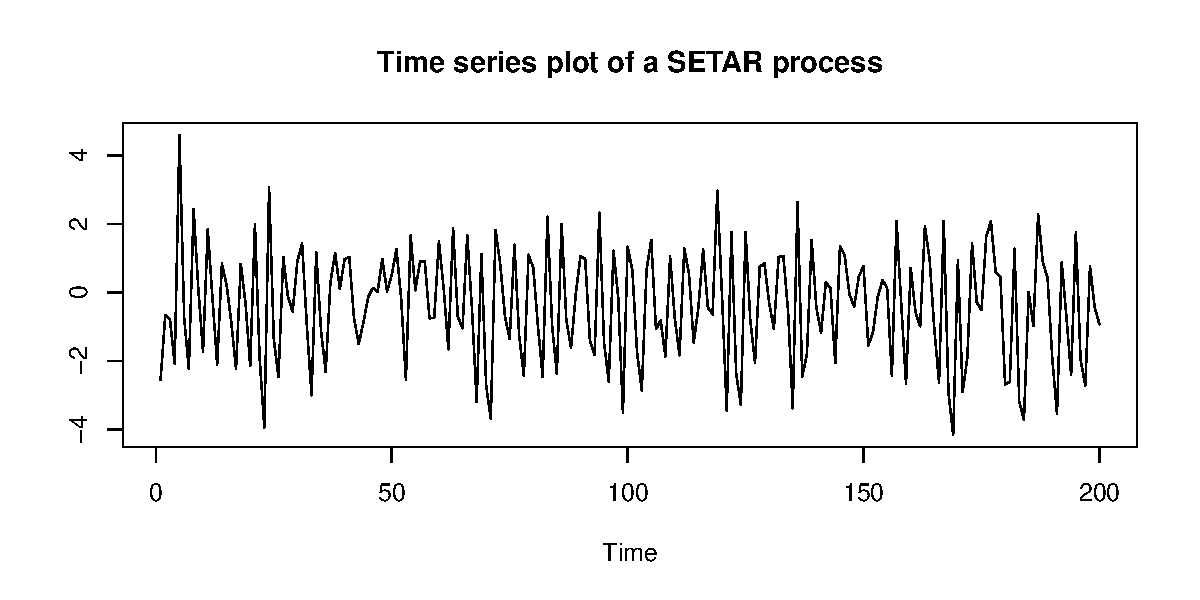
\includegraphics[width=3.5in]{SETAR}
\caption{Time series plot of the first 200 observations generated from the SETAR model in Equation (\ref{eqn:example}).}
\end{figure}


Estimation of the threshold value of the two-regime SETAR process can be done via the
function \code{uTAR.grid} or \code{uTAR} as illustrated below:
\begin{verbatim}
R> thr.est<- uTAR.grid(y = y$series, p1 = 2, p2 = 2, d = 2, thrV = NULL, thrQ = c(0,1),
+    Trim = c(0.1, 0.9), include.mean = T)
jst, jend:  200 1799 
Estimated Threshold:  0.1951103 
Regime 1:  
     Estimate Std. Error   t value     Pr(>|t|)
X1  1.0356009 0.04902797  21.12265 8.946275e-85
X2 -0.3017810 0.01581242 -19.08506 2.383743e-71
X3  0.4890477 0.02707987  18.05945 7.230880e-65
nob1 & sigma1:  1236 1.017973 
Regime 2:  
     Estimate Std. Error    t value     Pr(>|t|)
X1 -1.1352678 0.07222915 -15.717585 2.107275e-48
X2  0.5560001 0.03177212  17.499622 7.360494e-58
X3 -0.2122922 0.04641671  -4.573616 5.596852e-06
nob2 & sigma2:  762 1.034592 
  
The fitted TAR model ONLY uses data in the specified threshold range!!! 
Overal MLE of sigma:  1.012083 
Overall information criteria(aic,bic,hq):  0.02802025 0.03922205 0.03213331 

R> thr.est<- uTAR(y = y$series, p1 = 2, p2 = 2, d = 2, thrV = NULL, Trim = c(0.1, 0.9), k0 = 300,
+    include.mean = T, thrQ = c(0, 1))
Estimation of a SETAR model:  
Thresholds used:  0.1951103 
Estimation of regime:  1  with sample size:  1236 
       Estimate Std. Error   t value     Pr(>|t|)
cnst  1.0356009 0.04902797  21.12265 8.946275e-85
V2   -0.3017810 0.01581242 -19.08506 2.383743e-71
V3    0.4890477 0.02707987  18.05945 7.230880e-65
Sigma estimate:  1.017973 
Estimation of regime:  2  with sample size:  762 
       Estimate Std. Error    t value     Pr(>|t|)
cnst -1.1352678 0.07222915 -15.717585 2.107275e-48
V2    0.5560001 0.03177212  17.499622 7.360494e-58
V3   -0.2122922 0.04641671  -4.573616 5.596852e-06
Sigma estimate:  1.034592 
Overal AIC:  101.8515 
\end{verbatim}
\code{uTAR.grid} and \code{uTAR} share the following arguments: \code{y} is a vector of observed time seres, \code{p1} and \code{p2} are the AR order of regime 1 and regime 2, respectively, \code{d} is the delay, and \code{thrV} contains the external threshold variable $z_{t}$ which should have the same length as that of \code{y}. For SETAR models, \code{thrV} is not needed, i.e., setting \code{thrV} to NULL. \code{Trim} defines the lower and upper trimmings to control the minimum sample size in each regime and determine $[\underline{r}, \overline{r}]$ for estimation.  \code{include.mean} is a logical value for including
the constant term in each linear model. \code{k0} only used in the \code{uTAR} function controls the maximum sub-sample size when nested sub-sample search algorithm is used.


From the output, the estimated threshold value is 0.195, which is close to the true value 0.2. The estimated constant terms for regime 1 and regime 2 are 1.036 and -1.135, respectively.
The estimated AR coefficients for regime 1 and regime 2 are -0.302, 0.489, 0.556, and -0.212,
respectively.  The estimated standard deviations of the innovation processes in two regimes
are 1.018 and 1.035. As expected, all estimates are significant and close their true parameters.


Here we provide an incomplete list of the returned values of the functions \code{uTAR.grid} and \code{uTAR}:
\begin{itemize}\setlength\itemsep{-0.3em}
\item \code{residuals}: estimated innovations or residuals series.
\item \code{coefs}: a 2-by-($p+1$) matrix. The first row and second row show the estimated
coefficients in regime 1 and 2, respectively.
\item \code{sigma}: estimated covariances of the innovation process in regime 1 and regime 2.
\item \code{thr}: estimated threshold value.
\end{itemize}




Estimation of a multiple-regime TAR model with pre-specified threshold values  can be done by the
function \code{uTAR.est}. 
\begin{verbatim}
R> est <- uTAR.est(y = y$series, arorder = c(2, 2), thr = thr.est$thr, d = 2, output = FALSE)
\end{verbatim}
Here \code{aroder} is a row vector of positive integers containing the AR orders of all the regimes. \code{thr} contains the threshold values whose length should be the number of regimes minus 1. \code{output} is a logical value for printing out the estimation results with default being TRUE. The function \code{uTAR.est} returns the following components: \code{coefs} is a matrix with $m$ rows in which each row contains the estimated parameters for one regime, \code{sigma} contains the estimated innovation variances for different regimes, \code{residuals} collects the estimated innovations, and \code{sresi} shows the standardized residuals.



The following {R} code provides one-step-ahead prediction with function \code{uTAR.pred}.
\begin{verbatim}
R> pred <- uTAR.pred(model = est, orig = 2000, h = 1, iteration = 100, ci = 0.95,
+    output = TRUE)
Forecast origin:  2000 
Predictions: 1-step to  1 -step 
     step  forecast
[1,]    1 -1.559858
Pointwise  95  % confident intervals 
    step      Lowb      Uppb
int    1 -3.324043 0.6564724
\end{verbatim}
The output above shows that the one-step ahead prediction for $y_{2001}$ is -1.56. Various options in the function \code{uTAR.pred} provide users the flexibility to customize the forecasting origin with \code{orig}, forecast horizon with \code{h}, number of iterations with \code{iterations}, and confidence level with \code{ci}. The function \code{uTAR.pred} returns the prediction with \code{pred}. 


\medskip
The R function \code{thr.test} in the \pkg{NTS} package implements the $F$ test designed for SETAR models and proposed by \cite{tsay1989}. The test helps users detect the existence of nonlinear dynamics in the data. Below is the {R} code and output when we perform the nonlinearity tests with \code{thr.test}.
\begin{verbatim}
R> thr.test(y$series, p = 2, d = 2, ini = 40, include.mean = T)
SETAR model is entertained 
Threshold nonlinearity test for (p,d):  2 2 
F-ratio and p-value:  213.0101 1.511847e-119 
\end{verbatim}
\code{ini} is the initial number of data to start the recursive least square estimation. The output shows that $p$-value is very small, and they indicate that there is nonlinearity in the series \code{y\$series}.



\medskip
Back-testing can be used to evaluate the forecasting performance of a model and to
 conduct model comparison between different models. Back-testing for a univariate SETAR model is implemented through the function \code{backTAR} with syntax:
\begin{verbatim}
R> backTAR(model, orig, h = 1, iter = 3000)
\end{verbatim}
where \code{model} is an object returned by \code{uTAR} or \code{uTAR.est}, \code{h} is the forecast horizon, and \code{iter} controls the number of simulation iterations in prediction.

The function returns the model, out-of-sample rolling prediction errors and predicted states. It also
provides information  for model comparison. The following example shows the out-of-sample forecasting performance of SETAR models with delay 2 and 1, respectively. It shows that the root MSE,  mean absolute error, and biases of the model with delay 2 are all smaller than those of the model with delay 1. Hence, as expected, the model with delay 2 is preferred.

\begin{verbatim}
R> set.seed(11)
R> backTAR(est, 50, 1, 3000)
Starting forecast origin:  50 
1-step to  1 -step out-sample forecasts 
RMSE:  1.02828 
 MAE:  0.8172728 
Bias:  -0.001337478 
Performance based on the regime of forecast origins:  
Summary Statistics when forecast origins are in State:  1 
Number of forecasts used:  1204 
RMSEj:  1.029292 
 MAEj:  0.8172963 
Biasj:  0.00259177 
Summary Statistics when forecast origins are in State:  2 
Number of forecasts used:  746 
RMSEj:  1.026645 
 MAEj:  0.817235 
Biasj:  -0.007679051 
\end{verbatim}
\begin{verbatim}
R> thr.est2 <- uTAR.grid(y = y$series, p1 = 2, p2 = 2, d = 1, thrQ = c(0, 1),
+    Trim=c(0.1, 0.9), include.mean = T)
R> est2 <- uTAR.est(y = y$series, arorder = c(2, 2), thr = thr.est2$thr, d = 1)
R> set.seed(11)
R> backTAR(est2, 50, 1, 3000)
Starting forecast origin:  50 
1-step to  1 -step out-sample forecasts 
RMSE:  1.38731 
 MAE:  1.105443 
Bias:  -0.006635381 
Performance based on the regime of forecast origins:  
Summary Statistics when forecast origins are in State:  1 
Number of forecasts used:  1112 
RMSEj:  1.360347 
 MAEj:  1.090989 
Biasj:  0.2462278 
Summary Statistics when forecast origins are in State:  2 
Number of forecasts used:  838 
RMSEj:  1.4223 
 MAEj:  1.124622 
Biasj:  -0.3421769 
\end{verbatim}

The usage of functions for multivariate two-regime TAR models listed in Table \ref{table:TAR}, including \code{mTAR.sim}, \code{mTAR}, \code{mTAR.pred},  is similar to that of the univariate
counterpart functions discussed before. The only exception is that these multivariate functions
take different arguments to define the vector autoregressive(VAR) coefficients:
\begin{itemize}\setlength\itemsep{-0.3em}
\item \code{phi1, phi2}: VAR coefficient matrices of regime 1 and regime 2.
\item \code{sigma1, sigma2}: innovation covariance matrices of regime 1 and regime 2.
\item \code{c1, c2}: constant vectors of regime 1 and regime 2.
%\item \code{thrV}: values of the external threshold variable $z_{t}$, if any.
\item \code{delay}: two elements $(i,d)$ with "$i$" being the index of the component to be used as the threshold variable and "$d$" the delay for threshold variable. %If \code{thrV} is null, the model is self-exciting, and $d$ is threshold delay.
\end{itemize}


%Below is an example to illustrate how to generate a two-dimensional time series following a multivariate TAR model, to estimate the parameters, and to obtain a one-step-ahead prediction.

%\begin{verbatim}
%R> phi1 <- matrix(c(0.5, 0.7, 0.3, 0.2), 2, 2)
%R> phi2 <- matrix(c(0.4, 0.6, 0.5, -0.5), 2, 2)
%R> y <- mTAR.sim(nob = 100, thr = 0, phi1 = phi1, phi2 = phi2, sigma1 = matrix(
%+    c(1, 0, 0, 1), 2, 2), sigma2 = matrix(c(1, 0, 0, 1), 2, 2), c1 = c(0, 0),
%+    c2 = c(0, 0), delay = c(1, 1), ini = 500)
%R> est <- mTAR(y$series, p1 = 1, p2 = 1, delay = c(1, 1), k0 = 50)
%R> est.thr <- mTAR.est(y$series, arorder = c(1, 1), thr = 0, delay = c(1, 1))
%R> mTAR.pred(model = est, orig = 100, h = 1, iterations = 300, ci = 0.95,
%+    output = TRUE)
%\end{verbatim}

The function \code{mTAR} conducts the nested sub-sample search algorithm and provides different choices of criterion for threshold selection with the option \code{score}, namely (AIC, det(RSS)). It has less computational cost, but only applies to two-regime models. \code{mTAR.est} can handle multiple regimes. They both return a list of components with the estimated VAR coefficients in \code{beta}, estimated innovation covariance matrices in \code{sigma}, and estimated innovations in \code{residuals}.


\subsection{Analysis of non-Gaussian time series}
Autoregressive conditional mean (ACM) models are designed for time series of count data, starting with the autoregressive conditional Poisson models \citep{heinen2003}, and various extensions of ACM models were investigated. The \pkg{NTS} includes a function \code{ACMx} for the estimation of autoregressive conditional mean models with exogenous variables (ACMx models). Let $y_t$ be the time series of interest, $\mathbf{x}_t$ be a vector containing the exogenous variables, and ${\cal{F}}_t=\{ y_{t-1},y_{t-2},\ldots: \mathbf{x}_t, \mathbf{x}_{t-1},\ldots \}$. The ACMx models postulate
\[
y_t\mid {\cal F}_t \sim F(\cdot \mid \mu_t),
\]
where $\mu_t={\rm E}(y_t \mid {\cal F}_t)= \exp ({\mathbf x}_t' {\boldsymbol{\beta}})\lambda_t$,
and $\lambda_t$ follows the model
\[
\lambda_t=\omega+\sum_{i=1}^p \alpha_i\left[ \frac{y_{t-i}}{\exp(\mathbf{x}_{t-i}' \boldsymbol{\beta})}\right] +\sum_{j=1}^q \gamma_j \lambda_{t-j},
\]
$p$ and $q$ are nonnegative integers, $\omega>0$, and $\alpha_i$ and $\gamma_j$ are parameters satisfying certain conditions so that $\lambda_t$ is always positive and finite. The conditional distribution $F(y_t\mid {\cal F}_t)$ can be Poisson, negative binomial, or double Poisson \citep{tsay2018}.

The estimation of ACMx models is implemented via the function \code{ACMx} with syntax:
\begin{verbatim}
R> ACMx(y, order = c(1, 1), X = NULL, cond.dist = "po", ini = NULL)
\end{verbatim}
where \code{y} is the series of count data, \code{X} is the matrix of exogenous variables, \code{order} specifies the values for $p$ and $q$, \code{cond.dist} determines the conditional distribution with options: "po" for Poisson, "nb" for negative binomial, and "dp" for double Poisson,
and \code{ini} collects initial parameter estimates designed for use with "nb" or "dp".


We illustrate the function \code{ACMx} with an example below:
\begin{verbatim}
R> set.seed(12)
R> x <- rnorm(1000)*0.1
R> y <- matrix(0, 1000, 1)
R> lambda <- matrix(0, 1000, 1)
R> for (i in 2:1000){
+    lambda[i] <- 2 + 0.2*y[i-1]/exp(x[i-1]) + 0.5*lambda[i-1]
+    set.seed(i)
+    y[i] <- rpois(1, exp(x[i]) * lambda[i])
+  }
R> ACMx(y,order = c(1, 1), x, "po")
Initial estimates:  1.061758 1.737901 0.05 0.5 
loB:  -1.061758 1e-06 1e-06 1e-06 
upB:  3.185275 19.11691 0.5 0.999999 
Maximized log-likehood:  -2372.64 

Coefficient(s):
       Estimate  Std. Error  t value   Pr(>|t|)    
beta  1.0568837   0.1274883  8.29004 2.2204e-16 ***
omega 2.6589289   0.5509761  4.82585 1.3941e-06 ***
alpha 0.1594231   0.0266118  5.99070 2.0894e-09 ***
gamma 0.4428811   0.0904537  4.89622 9.7698e-07 ***
---
Signif. codes:  0 '***' 0.001 '**' 0.01 '*' 0.05 '.' 0.1 ' ' 1
\end{verbatim}

Here a time series following ACMx model with Poisson conditional distribution, order (1,1), $\beta=1$, $\omega=2$, $\alpha=0.2$ and $\gamma=0.5$ is generated. The {R} output reports the estimated coefficients which are all significant and close to their true values.

\subsection{Functional time series}
Functional time series analysis has received much attention since the pioneering work of \cite{bosq2000}, and has been widely applied in many fields, including environmental science \citep{hormann2010}, social science \citep{hyndman2000}, and finance \citep{diebold2006,horvath2013}. \cite{liu2016functional} proposed a new class of models called the convolutional
functional autoregressive (CFAR) models, which has an intuitive
and direct interpretation of the dynamics of a stochastic process. The
\pkg{NTS} encompasses functions to implement the method proposed by \cite{liu2016functional}.

Before presenting these {R} functions, we briefly introduce the CFAR model and its estimation procedure. A sequence of square integrable random functions $\{X_t\mid t=1,\ldots, T\}$ defined on $[0,1]$ follows a convolutional functional autoregressive (CFAR) model of order $p$ if
\[
X_t(s)=\sum_{i=1}^p \int_0^1 \phi_i(s-u)X_{t-i}(u)du +\epsilon_t(s), \quad s\in[0,1],
\]
where $\phi_i(\cdot)$ are square integrable and defined on $[-1,1]$ ($i=1,\ldots,p$) and are called the convolutional coefficient functions, and $\epsilon_t$ are i.i.d. Ornstein-Uhlenbeck (O-U) processes defined on [0,1] satisfying the stochastic differential equation, $d\epsilon_t(s)=-\rho \epsilon_t(s)ds+\sigma dW_s$, $\rho>0$, and $W_s$ is a Wiener process.

In practice, $X_t(\cdot)$ is usually observed only at discrete points, $s=i/N$, $i=0,\ldots N$ for time $t=1,\ldots T$. \cite{liu2016functional} recovers the function $X_t(\cdot)$ by linear interpolation,
\[
\widetilde{X}_t(s)=\frac{(s_i-s)X_t(s_{i-1})+(s-s_{i-1})X_t(s_i)}{1/N}, \mbox{ for } s_{i-1}\leq s< s_i,
\]
and approximates $\phi_i(\cdot)$ by cubic B-splines,
\[
\phi_i(\cdot) \approx \widetilde{\phi}_i(\cdot)=\sum_{j=1}^k {\beta}_{k,i,j}B_{k,j}(\cdot), \mbox{ for } i=1,\ldots p,
\]
where $\{B_{k,j},j=1,\ldots,k\}$ are uniform cubic B-spline basis functions with $k$ degrees of freedom.

With the above approximation, the B-spline coefficients $\boldsymbol{\beta}=\{{\beta}_{k,i,j}\}$, $\rho$, and $\sigma^2$ can be estimated by maximizing the approximated log-likelihood function. Specifically
\[
(\hat{{\boldsymbol{\beta}}},\, \hat{\rho},\, \hat{\sigma}^2)=\arg \max Q(\boldsymbol{\beta}, \rho,\sigma^2),
\]
where
\[
Q(\boldsymbol{\beta}, \rho,\sigma^2)=C+\frac{(N+1)(T-p)}{2}\ln \left(\frac{\pi \sigma^2}{\rho}\right)-\frac{N(T-p)}{2}\ln (1-e^{-2\rho/N}) -\frac{1}{2}\sum_{t=1}^T \mathbf{e}_t' \Sigma^{-1} \mathbf{e}_t,
\]
where $C$ is a constant, $\mathbf{e}_t=(e_{t,1},\ldots e_{t,N})'$, and $e_{t,i}=X_t(i/N)-\sum_{j=1}^k {\beta}_{k,i,j} \int_0^1 B_{k,j}(s-u) \widetilde{X}_t(s)du$.

The convolutional functions are estimated by
\[
\hat{\phi}_i(\cdot)=\sum_{j=1}^k \hat{\beta}_{k,i,j}B_{k,j}(\cdot).
\]

In the \pkg{NTS} package, model specification and estimation of a CFAR process can be carried out by the functions \code{F\_test\_cfar} and \code{est\_cfar} with the syntax:
\begin{verbatim}
R> F_test_cfar(f, p.max = 6, df_b = 10, grid = 1000)
R> est_cfar(f, p = 3, df_b = 10, grid = 1000)
\end{verbatim}
The observed functional time series is stored in \code{f}, which is a $T$-by-$N$ matrix, where $T$ is the length of time, and $N$ is the number of discrete observations of the functional data at a given time period minus 1. \code{p} specifies the CFAR order.  \code{df\_b} determines the degrees of freedom $k$ for
the natural cubic splines, and \code{grid} is the number of grid points used to construct the functional time series and noise process.

The function \code{F\_test\_cfar} returns the test statistics and the $p$-values for a sequence of $F$-tests with $H_0: \phi_k(\cdot)=0, \phi_i(\cdot)\neq 0, i=1\ldots, k-1$ versus $H_a: \phi_i(\cdot) \neq 0, i=1,\ldots,k$ for  $k=1,\ldots$, \code{p.max}. The function \code{est\_cfar} returns the following values: \code{phi\_coef} collects the estimated spline coefficients $\hat{\beta}_{k,i,j}$ for the convolutional function(s) which is a $(\texttt{df\_b}+1)\times p$ matrix, and \code{phi\_func} contains the estimated convolutional function values which is a $(2\times \texttt{grid}+1) \times p$ matrix. \code{rho} is the estimated $\rho$ in the O-U process, and \code{sigma} is estimated standard deviation of the noise process, respectively.


The function \code{g\_cfar} in the \pkg{NTS} package generates a CFAR process with argument \code{tmax} being the length of time, \code{rho} is the parameter for the O-U process, \code{sigma} is the standard deviation of the O-U process, \code{phi\_list} is the convolutional function(s), and \code{ini} is the burn-in period. It returns a list with two components. One is \code{cfar}, a \code{tmax}-by-(\code{grid}+1) matrix following the CFAR(p) model, and the other one \code{epsilon} is the innovation at time \code{tmax}.
Function \code{p\_cfar} provides the forecasts of a CFAR model with argument \code{model} as a result of an \code{est\_cfar} fit and argument \code{m} as the forecasting horizon.

Let us consider a CFAR(1) process with the following convolutional coefficient function
\begin{align}\label{cfar}
\phi(s)=\frac{10}{\sqrt{2\pi }}e^{-50s^2}, \quad s\in[-1,1],
\end{align}
where $\phi(\cdot)$ is the probability density function of a Gaussian random variable with mean 0 and standard deviation 0.1 truncated in the interval $[-1,1]$. For the O-U process, $\rho=5$ and its standard deviation is 1. The following {R} code simulates such a CFAR(1) process specified in Equation (\ref{cfar}) with $N=100$, $T=1000$, and burn-in period 100, conducts an $F$ test, performs the estimation procedure,
and provides a one-step ahead prediction.

\begin{verbatim}
R> phi_func <- function(x){
+    return(dnorm(x, mean = 0, sd = 0.1))
+  }
R> t=1000; N=50;
R> x=g_cfar(t, rho=5, phi_func, sigma=1, ini=100)
R> f=x$cfar[,seq(1,1001,1000/N)]
R> F_test_cfar(f, p.max=2, df_b=10, grid=1000)
Test and p-value of Order 0 vs Order 1:  
[1] 1368.231    0.000
Test and  p-value of Order 1 vs Order 2 :  
[1] 0.6848071 0.7544262
R> model=est_cfar(f, p=1, df_b=10, grid=1000)
R> print(c(model$rho, model$sigma))
[1] 4.940534 1.005315
R> pred=p_cfar(model, f, m = 3)
\end{verbatim}


\begin{figure}[t!]
\centering
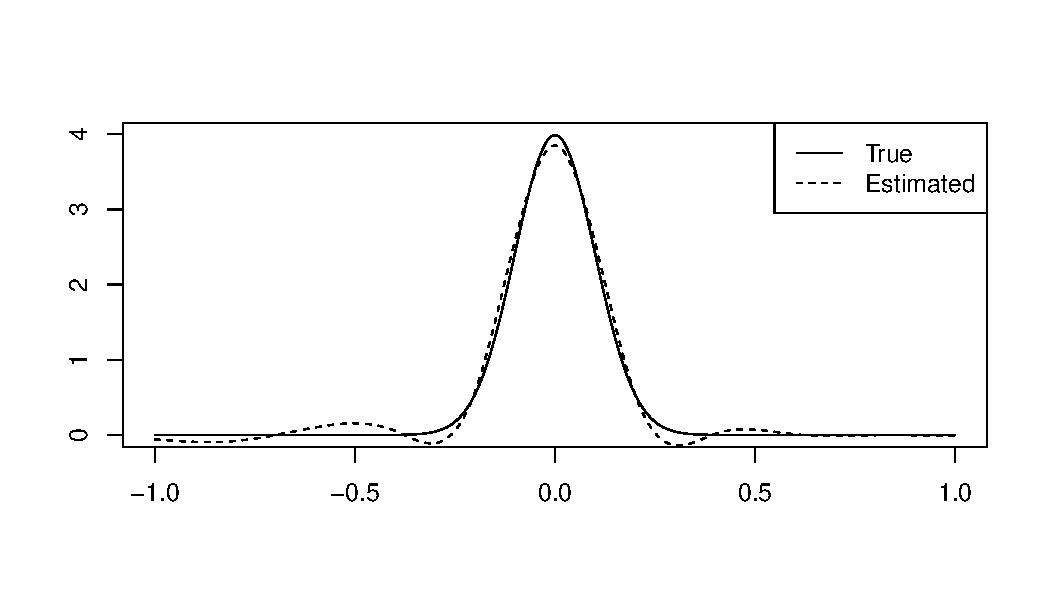
\includegraphics[width=3.5in]{article-cfar_plot}
\caption{True convolution function $\phi(\cdot)$ and estimated convolution function $\hat{\phi}(\cdot)$.}
\end{figure}



From the output, the $p$-values for $F$ tests suggest that we choose CFAR(1) model for the data. $\hat{\rho}=4.941$ and the standard deviation of the noise process is estimated as $1.005$, and they are both close to their true values.
 Figure 2 plots the estimated convolutional function (dashed line) and true function $\phi(\cdot)$ (solid line). It can be seen that \code{est\_cfar} performs well.
 
 
\code{F\_test\_cfarh} and \code{est\_cfarh} in \pkg{NTS} can deal with heteroscedasticity and irregular observation locations with following arguments: \code{weight} is the heteroscedasticity weight function of the noise process with \code{grid}+1 elements, \code{num\_obs} is a $t$-by-$1$ vector and collects the numbers of observations at different times, and \code{x\_pos} is a $t$-by$(N+1)$ matrix and shows the observation locations, where $(N+1)$ is the maximum number of observation at a time. The R code below will yield the same results as the previous one does. Hence, the output is omitted.
\begin{verbatim}
R> num_obs = rep(N+1, t); x_pos = matrix(rep(seq(0, 1, 1/N), each = t), t, N+1);
R> weight0=function(x){return(rep(1,length(x)))}
R> F_test_cfarh(f, weight0,p.max=2, df_b=10, grid=1000,num_obs, x_pos)
R> modelh=est_cfarh(f, weight0, p=1, df_b=10, grid=1000, num_obs,x_pos)
\end{verbatim}


\section[State-Space Modelings via Sequential Monte Carlo Methods] {State-Space Modelings via Sequential Monte Carlo Methods}



It is challenging to derive analytic solutions for filtering or smoothing of
nonlinear or non-Gaussian state-space models.  The sequential Monte Carlo (SMC) approach
(or particle filer) fully utilizes the dynamic nature of the model, and is an effective way to solve such complex problems \citep{tsay2018}. Consider the state-space model:
\begin{align*}
\begin{array}{lccc}
\mbox{State equation:}	&x_t=s_t(x_{t-1},\epsilon_t) &\mbox{ or } &x_t \sim q_t(\cdot \mid x_{t-1}),\\
\mbox{Observation equation:}&y_t=h_t(x_t, e_t) &\mbox{ or } & y_t\sim f_t(\cdot \mid x_t),
\end{array}
\end{align*}
where $x_t$ is the unobservable state variable and $y_t$ is the observation ($t=1,\ldots T$).
The underlying states evolve through the known function $s_t(\cdot)$ and the state innovation
 $\epsilon_t$, following a known conditional distribution $q_t(\cdot)$. The information on the underlying states is observed indirectly through $y_t$ via the known function $h_t(\cdot)$ and with
 observational noise $e_t$. The function $h_t(\cdot)$ and the distribution of $e_t$ are known with
 possibly unknown parameters to be estimated.

In general, there are four main statistical inference objectives associated with a state-space model:
\begin{enumerate}
\item Filtering: obtain the marginal posterior distribution of the current state $x_t$ given the entire history of the observations up to the current time, i.e., $p(x_t \mid y_1, \ldots y_t)$.
\item Prediction: obtain the marginal posterior distribution of the future state given the
current available information,  that is,  $p(x_{t+1}\mid y_1,\ldots, y_t)$.
\item Smoothing: obtain the posterior distribution of the state at the time $t$ given the entire available information, that is, $p(x_{t} \mid y_1,\ldots, y_T)$.
\item Likelihood and parameter estimation. SMC uses a set of weighted samples $\{x_t^{(j)},w_t^{(j)}\}$ to approximate the distribution $p(x_1,\ldots, x_t \mid y_1,\ldots, y_t)$.
\end{enumerate}

SMC is a recursive procedure with three components:
\begin{itemize}
\item {\bf Propagation step}: At time $t$ for $j=1,\ldots, m$: draw $x_t^{(j)}$ from a trial distribution $g_t(x_t \mid {\mathbf x}_{t-1}^{(j)},y_t)$, where $m$ is the Monte Carlo sample size. Attach it to ${\mathbf x}_{t-1}^{(j)}$ to form ${\mathbf x}_{t}^{(j)}=({\mathbf x}_{t-1}^{(j)}, x_t^{(j)})$. Compute the new weight for $x_{t}^{(j)}$.
\item {\bf Resampling step}: Obtain a new set of indices $\{I_1, \ldots, I_m\}$, where $I_k\in \{1, \ldots, m \}$ according to a set of priority scores $\alpha_t^{(j)}$, $j=1,\ldots, m$. Replace the sample with $\{x_t^{(I_j)}, \hat{w}_t^{(I_j)}=w^{(I_j)}/\alpha^{(I_j)}\}$.
\item {\bf Inference Step}: Estimation of ${\rm E}_{\pi_t}[(h({\mathbf x}_t)]$ for some integrable function $h(\cdot)$ using the generated weighted samples $({\mathbf x}_t^{(j)}, w_t^{(j)})$, $j=1,\ldots,m$, where $\pi_t(\cdot)$ is the target distribution. 
\end{itemize}
The selection of the propagation trial distribution $g_t(x_t\mid {\mathbf x}_{t-1},y_t)$ plays a key role
for an efficient implementation of SMC.

Since the efficiency of SMC is determined by the variance of weight distribution, one would naturally want to choose $g_t(\cdot)$ so that the incremental weight is as close to a constant as possible. \cite{LiuChen1995, LiuChen1998} proposed the trial distribution
\[
g_t(x_t\mid {\mathbf x}_{t-1})=p(x_t\mid {\mathbf x}_{t-1},{\mathbf y}_t)\quad  \propto\quad  q_t(x_t\mid x_{t-1})f_t(y_t\mid x_t).
\]
The proposed distribution utilizes information from both the state and observation equations, hence is termed a full information propagation step.

\noindent{\bf Algorithm: Full information propagation step}\\
At time $t$, for $j=1,\ldots,m$:
\begin{enumerate}
\item Draw $x_t^{(j)}$ from the local posterior distribution,
\begin{align*}
g_t(x_t\mid x_{t-1}^{(j)}, y_t)=p(x_t \mid x_{t-1}^{(j)},y_t)\, \propto\,  f_t(y_t\mid x_t)q_t(x_t \mid x_{t-1}^{(j)}).
\end{align*}
\item Compute the incremental weight
\[
u_t^{(j)}=\int f_t(y_t \mid x_t) q_t(x_t \mid x_{t-1}^{(j)})dx_t
\]
and the new weight $w_t^{(j)}=w_{t-1}^{(j)}u_t^{(j)}$.
\end{enumerate}
\cite{gordon1993} and \cite{kitagawa1996} used the state equation only for the trial distribution $g_t(\cdot)$. The implementation is called bootstrap filter.

\noindent{\bf Algorithm: Propagation step in bootstrap filter}\\
At time $t$, for $j=1,\ldots,m$:
\begin{enumerate}
\item Draw $x_t^{(j)}$ using the state equation
\begin{align*}
x_t^{(j)} \sim q_t(x_t \mid x_{t-1}^{(j)}).
\end{align*}
This is the same as generating $\epsilon_t^{(j)}$ first and obtaining $x_t^{(j)}=s_t(x_{t-1}^{(j)}, \epsilon_t^{(j)})$.
\item Compute the new weight $w_t^{(j)}=w_{t-1}^{(j)}f_t(y_t\mid x_t^{(j)})$.
\end{enumerate}

The bootstrap filter is easy to implement and computational inexpensive when $\epsilon_t^{(j)}$ is easy to generate. However, it may not be efficient because information on the current observation $y_t$ is not fully utilized.

The independent particle filter of \cite{lin2005} uses the observation equation only as the trial distribution. It shows better performance when the state dynamics $q_t(\cdot)$ is weak and the information from the observation $f_t(\cdot)$ is strong.

\noindent{\bf Algorithm: Propagation step in independent particle filter}\\
At time $t$, for $j=1,\ldots,m$:
\begin{enumerate}
\item Draw $x_t^{(j)}$ using the observation equation $g_t(x_t\mid y_t)\, \propto\, f_t(y_t \mid x_t)$.
\item Select $L$ different permutations of $\{1,\ldots,m\}: K_l=\{k_{l,1},\ldots, k_{l,m}\}$, $l=1,\ldots,L$. Compute the incremental weight
\[
u_t^{(k_{l,j},j)}\propto q_t(x_t^{(j)}\mid x_{t-1}^{(k_{l,j})})
\]
for each permutation. Compute the multiple matching weight
\[
w_t^{(j)}=\frac{1}{L} \sum_{l=1}^L u_t^{(k_{l,j},j)} w_{t-1}^{(k_{l,j})}.
\]
\end{enumerate}

It is shown that the variance of the weight distributions stochastically increases over time. Continuing to propagate the samples with small weights forward is a waste of computational resources since inference is based on weighted average of the samples. One solution is to use resampling schemes to duplicate the importance samples and to eliminate the ones with low weights. Hence resampling steps are essential in SMC implementations. Another issue to consider is how to make inference as efficient as possible. Rao-Blackwellization is one of the effective tools that can be used.

Smoothing is another important inference to make when we analyze data with state-space models. Delayed estimation (e.g. making inference on $p(x_{t-d}\mid y_1,\ldots,y_t)$) is a special case of smoothing. It can be achieved simply by using the weighted sample $\{(x_{t-d},w_t^{(j)})\}$. However, when $d$ is large, this sampling approach does not work well because resampling reduces the number of unique ancestors and thus increases the estimation errors. A more efficient algorithm is to calculate the backward smoothing weights, after obtaining the forward filtering weighted samples $\{(x_t^{(j)},w_t^{(j)}), j=1,\ldots,m\}$. The resulting weighted sample $\{(x_t^{(j)}, \tilde{w}_t^{(j)}), j=1,\ldots,m\}$ is properly weighted.

\noindent{\bf Algorithm: Weight marginalization SMC smoother}\\
Let $\tilde{w}_T^{(j)}=w_T^{(j)}, j=1,\ldots,m$. For $t=T-1,T-2,\ldots, 1$ and $j=1,\ldots, m$: \\
Calculate
\[
\tilde{u}_t^{(j)}=\sum_{i=1}^m \frac{q_{t+1}(x_{t+1}^{(i)}\mid x_t^{(j)})}{\sum_{k=1}^m q_{t+1}(x_{t+1}^{(i)}\mid x_t^{(k)}) w_t^{(k)}} \tilde{w}_{t+1}^{(i)}
\]
and the smoothing weight $\tilde{w}_t^{(j)}=w_t^{(j)}\tilde{u}_t^{(j)}$.

Table \ref{table:SMC} lists functions in \pkg{NTS} that implement the aforementioned SMC procedures.
\begin{table}[h]
\begin{center}
\footnotesize
\caption{List of {R} functions about SMC in package \pkg{NTS}}
\begin{tabular}{l| l|  l}\hline
Usage	&Function	&description\\ \hline
Generic function&\code{SMC}		&SMC method with delay but not using a full information propagation step\\
&\code{SMC.Smooth}	&SMC smoothing method\\
&\code{SMC.Full}		&SMC method using a full information propagation step\\
&\multirow{2}{*}{\code{SMC.Full.RB}} &SMC method using a full information propagation step with\\
&&Rao-Blackwellization estimate and no delay\\  \hline
\end{tabular}\label{table:SMC}
\end{center}
\end{table}

The \code{SMC} function can be called by:
\begin{verbatim}
R> SMC(Sstep, nobs, yy, mm, par, xx.init, xdim, ydim, resample.sch,
+    delay = 0, funH = identity)
\end{verbatim}
The following arguments need to be specified for \code{SMC}.
\begin{itemize}\setlength\itemsep{-0.3em}
\item \code{Sstep}: A function that performs one step propagation using a proposal distribution. Its input variables include (\code{mm, xx, logww, yyy, par, xdim, ydim}), where  \code{xx} and \code{logww} are the prior iteration samples and their corresponding log weights, and \code{yyy} is the observation at current time step. It returns a list that contains \code{xx} (the sample $x_t$) and \code{logww} (their corresponding log weights).
\item \code{nobs}: the number of observations, $T$.
\item \code{yy}: the observations with $T$ columns and \code{ydim} rows.
\item \code{mm}: the Monte Carlo sample size $m$.
\item \code{par}: a list of parameter values to pass to \code{Sstep}.
\item \code{xx.init}: the initial samples of $x_0$.
\item \code{xdim, ydim}: the dimension of the state variable $x_t$ and the observation $y_t$.
\item \code{resample.sch}: a binary vector of length \code{nobs}, reflecting the resampling schedule. \\
\code{resample.sch[i]=1} indicates resample should be carried out at step $i$.
\item \code{delay}: the maximum delay lag for delayed wighting estimation. Default is zero.
\item \code{funH}: a user supplied function $h(\cdot)$ for estimating ${\rm E}(h(x_t)\mid y_{t+d})$. Default is identify function for estimating the mean with no delay. The function should be able to take vector or matrix as input and operates on each element of the input.
\end{itemize}
The function returns \code{xhat}, an array with dimensions (\code{xdim,nobs,delay+1}) and the scaled log-likelihood value \code{loglike}. The functions \code{SMC.Smooth}, \code{SMC.Full} and \code{SMC.Full.RB} have similar inputs and outputs, except that \code{SMC.Smooth} needs another input function for the backward smoothing step and \code{funH} is a function for estimating ${\rm E}(h(x_t)\mid y_1,\ldots, y_{T})$.

Here is an example demonstrating how to implement SMC methods using the \pkg{NTS} package.
We consider the following simple model,
\begin{align*}
x_t&=x_{t-1}+\sigma_w w_t,\\
y_t&=x_t+\sigma_v v_t,
\end{align*}
where $w_t \sim N(0,1)$, $v_t\sim N(0,1)$, and they are independent.

The simulated samples can be generated using the following function.

\begin{verbatim}
R> simuRW <- function(nobs, ssw, ssv, xx0){
+    xx = 1:nobs
+    ww = rnorm(nobs)*ssw
+    vv = rnorm(nobs)*ssv
+    xx[1] = xx0 + rnorm(1)
+    for(i in 2:nobs){
+      xx[i] = xx[i-1] + ww[i]
+    }
+    yy = xx + vv
+    return(list(xx = xx, yy = yy))
+  }
\end{verbatim}

The following statements are user generated functions for various sequential importance sampling
 step implementations.

\begin{verbatim}
R> SISstep.RW.Full <- function(mm, xx, logww, yyy,par, xdim, ydim, resample.sch){
+    ssw2 = par$ssw**2; ssv2 = par$ssv**2
+    tau2 = 1/(1/ssw2 + 1/ssv2); tau = sqrt(tau2)
+    mu = (xx/ssw2 + yyy/ssv2)*tau2
+    logww = logww - xx**2/2/ssw2 - yyy**2/2/ssv2 + mu**2/2/tau2
+    logww = logww - max(logww)
+    if(resample.sch == 0) r.index = rep(0, mm)
+      if(resample.sch == 1){
+          ww = exp(logww)
+          ww = ww/sum(ww)
+          r.index = sample.int(mm, size = mm, replace = T, prob = ww)
+          xx = xx[r.index]
+          mu = mu[r.index]
+          logww = logww*0
+      }
+      xx = mu + rnorm(mm)*tau
+      return(list(xx = xx, logww = logww, r.index = r.index))
+   }
R> SISstep.RW.B <- function(mm, xx, logww, yyy, par, xdim, ydim){
+    ee = rnorm(mm)*par$ssw
+    xx = xx + ee
+    logww = logww + (xx*yyy - xx**2/2)/par$ssv**2
+    logww = logww - max(logww)
+    return(list(xx = xx, logww = logww))
+  }
R> SISstep.RW.I <- function(mm, xx, logww, yyy, par, xdim, ydim){
+    ee = rnorm(mm)*par$ssv
+    xx.new = matrix(yyy - ee, nrow = 1)
+    logww = logww - (xx.new - xx)**2/2/par$ssw**2
+    logww = logww - max(logww)
+    return(list(xx = xx.new, logww = logww))
+  }
\end{verbatim}

Now we are ready to run the simulation study with sample size $T=200$, Monte Carlo sample size $m=100$, and $\sigma_w=\sigma_v=1$.

\begin{verbatim}
R> simu <- simuRW(nobs = 200, ssw = 1, ssv = 1, xx0 = 0)
R> out1<- SMC.Full(SISstep.RW.Full, nobs = 200, yy = simu$yy, mm = 100,
+    par = list(ssw = 1, ssv = 1), xx.init = rnorm(100), xdim = 1, ydim = 1,
+    resample.sch = rep(1, 200), delay = 0)
R> out2 <- SMC(SISstep.RW.B, nobs = 200, simu$yy, mm = 100, par = list(ssw = 1,
+    ssv = 1), xx.init = rnorm(100), xdim = 1, ydim = 1, resample.sch = rep(1,
+    200), delay = 0)
R> out3 <- SMC(SISstep.RW.I, nobs = 200, simu$yy, mm = 100, par = list(ssw = 1,
+    ssv=1), xx.init = rnorm(100), xdim = 1, ydim = 1, resample.sch = rep(1,
+    200), delay = 0)
\end{verbatim}



\begin{table}[h]
\begin{center}
\caption{Filtering mean squared errors for different methods}
\begin{tabular}{l| c| ccc}\hline
$\sigma_w^2=1$, $\sigma_v^2=1$	&Kalman filter	&Full &Bootstrap	&Independent\\ \hline
every step		&0.601	&0.608	&0.615   &0.615	\\
every 5 steps	&		    &0.612	&0.641	  &0.665\\
no resample	  &		    &0.938	&13.88	  &1.597\\ \hline
$\sigma_w^2=1$, $\sigma_v^2=4$ &&&&\\ \hline
every step		&4.018	&4.143	&4.149	  &5.092\\
every 5 steps	&		    &4.078	&4.153	  &10.272\\
no resample	  &		    &6.809	&12.604	  &27.189\\ \hline
$\sigma_w^2=4$, $\sigma_v^2=1$ &&&&\\ \hline
every step		&1.023	&1.032	&1.031		  &1.031\\
every 5 steps	&		    &1.034	&2.972		  &1.031\\
no resample	  &		    &1.153	&197.725		&1.296\\ \hline
\end{tabular}\label{tbl:SMC}
\end{center}
\end{table}


To compare the performance of different methods under various conditions, we run 50 simulations and vary the values of $\sigma_w$ and $\sigma_v$ and resampling schedules. Table \ref{tbl:SMC} reports the mean squared errors for all methods. Since Kalman filter is the optimal and most efficient approach when the model is linear and Gaussian, we use it as the baseline for comparison. From Table \ref{tbl:SMC} it is seen that
the full information proposal distribution yields the smallest MSE among all SMC methods and is quite close to that of Kalman filter. The bootstrap filter outperforms the independent filter when the observational noise is relatively large ($\sigma_w^2=1$ and $\sigma_v^2=4$). On the other hand, when the observational noise is relatively small, the independent filter outperforms the bootstrap filter.


The following code shows how to run the simulation study with sample size $T=200$, Monte Carlo sample size $m=100$, and $\sigma_w=\sigma_v=1$ for SMC smoothing. Table \ref{tbl:smooth} shows the performance of using bootstrap filter and independent filter in SMC smoother with 50 simulations. It has a similar pattern to that of Table \ref{tbl:SMC}.
\begin{verbatim}
R> SISstep.Smooth.RW <- function(mm, xxt, xxt1, ww, vv, par){
+    ssw = par$ssw
+    uu = 1:mm
+    aa = 1:mm
+    for(i in 1:mm){
+      res = (xxt[i] - xxt1)/ssw
+      aa[i] = sum(exp(- res**2/2)*ww)
+    }
+    for(j in 1:mm){
+      res = (xxt - xxt1[j])/ssw
+      uu[j] = sum(exp(- res**2/2)*vv/aa)
+    }
+    vv = ww*uu
+    return(list(vv = vv))
+  }
R> out4 <- SMC.Smooth(SISstep.RW.B, SISstep.Smooth.RW, nobs = 200, simu$yy,
+    mm = 100, par = list(ssw = 1, ssv = 1), xx.init = rnorm(100), xdim = 1,
+    ydim = 1, resample.sch = rep(1, 200))
R> out5 <- SMC.Smooth(SISstep.RW.I, SISstep.Smooth.RW, nobs = 200, simu$yy,
+    mm = 100, par = list(ssw = 1, ssv = 1), xx.init = rnorm(100), xdim = 1,
+    ydim = 1, resample.sch = rep(1,200))
\end{verbatim}

\begin{table}
\begin{center}
\caption{Smoothing mean squared errors for different methods}
\begin{tabular}{l| c| ccc}\hline
$\sigma_w^2=1$, $\sigma_v^2=1$	&Bootstrap	&Independent\\ \hline
every step		  ` &0.618		  &0.639		\\
every 5 steps	    &0.601			&0.686	\\
every 10 steps	  &0.749			&0.769	\\ \hline
$\sigma_w^2=1$, $\sigma_v^2=4$ &&&&\\ \hline
every step		    &4.147		  &6.04	\\
every 5 steps	    &3.745		  &10.608	\\
every 10 steps	  &3.492		  &14.135	\\ \hline
$\sigma_w^2=4$, $\sigma_v^2=1$ &&&&\\ \hline
every step		    &1.169		  &1.031	\\
every 5 steps	    &2.933		  &1.033	\\
every 10 steps    &8.005			&1.035	\\ \hline
\end{tabular}\label{tbl:smooth}
\end{center}
\end{table}

\section{Conclusion}
The paper introduced the {R} package \pkg{NTS} which offers a broad collection of functions for the analysis of nonlinear time series data. We briefly review various nonlinear time series models, including threshold autoregressive models, autoregressive conditional mean models with exogenous variables, convolutional functional autoregressive models, and state-space models. The associated estimation, identification, and forecasting procedures are discussed. The \pkg{NTS} provides computational tools to fit these models, to evaluate their performance, and to provide predictions. Furthermore, the functions can be used, extended, and modified within the package to analyze larger univariate/multivariate, Gaussian/non-Gaussian time series. These features enable users to carry out a comprehensive and complex analysis of time series without the constraints from software availability.







\bibliography{liu}

\address{Xialu Liu\\
  Department of Management Information Systems\\
  San Diego State University\\
  5500 Campanile Drive, San Diego, CA 92182\\
  USA\\
  \email{xialu.liu@sdsu.edu}}

\address{Rong Chen\\
  Department of Statistics\\
  Rutgers University\\
  57 US Highway 1, New Brunswick, NJ 08901\\
  USA\\
  \email{rongchen@stat.rutgers.edu}}

\address{Ruey Tsay\\
  Booth School of Business\\
  University of Chicago\\
  5801 E Ellis Ave, Chicago, IL 60637\\
  USA\\
  \email{ruey.tsay@chicagobooth.edu}}
  
\noindent Chen's research is supported in part by
National Science Foundation grants DMS-1503409, DMS-1737857, IIS-1741390 and CCF-1934924.
